\subsection{Project Functionality}
The following sections provide instruction for using the Hephaestus software.

\subsubsection{Project Structure}
The Hephaestus project's software is divided into a series of modules called
\textit{phases}.
The software must wholly complete each phase before it moves on to the next
phase.
The one exception to this rule is if an error event occurs.
In this case, the phase returns an error code, and immediately enters the 
\textit{safety} phase.
Each phase is responsible for one operation of the experiment.
For example, the \textit{observation} phase in responsible for turning on the
camera and panning it around and the \textit{safety} phase is responsible for 
resolving any error conditions present and safely retracting the arm for 
reentry.

\subsubsection{Theory of Operation}
When the system powers on, it immediately enters the \textit{idle} phase.
After completion of each phase, it moves on to the next logical phase.
The system halts in the \textit{off} phase.
If an error occurs in any phase, it aborts the current phase and enters the
\textit{safety} phase.

Each phase is described as follows:
\begin{enumerate}
	\item{\textbf{Idle phase}}

	This phase does nothing until a signal is received indicating that the
	rocket has reached \gls{apogee} and the experiment may start.

	\item{\textbf{Observation phase}}

	This phase turns on the camera and performs a 360° pan.
	After completing the pan, it points the camera toward the arm to record the
	rest of the experiment.

	\item{\textbf{Science phase}}

	The Science phase is responsible for the motion of the arm in space.
	This phase powers on the motors and runs them along the path noted in the configuration 
	space. The configuration space is pre-computed but is loaded into program memory for use on 
	orbit.

	\item{\textbf{Retract phase}}

	The retract phase powers off all the motors except for the motor powering the lower deck plate. Once all motors powering the arm
	and camera have been disabled, the deckplate motor pulls in the arm body. This phase is reached if there is an error after the 
	Science phase or if the end of the \gls{apogee} period is reached.

	\item{\textbf{Off phase}}

	The off phase merely terminates the program execution.

	\item{\textbf{Safety phase}}

	The safety phase is responsible for resolving and/or mitigating any errors
	that occur during any of the other phases.
	This phase is only reached if any of the other phases returns an error
	code.
	The current implementation of the safety phase simply attempts to retract
	arm and terminate, but this could be extended in future projects to attempt to resolve
	problems and resume the program.
\end{enumerate}

\subsubsection{Block Diagram}
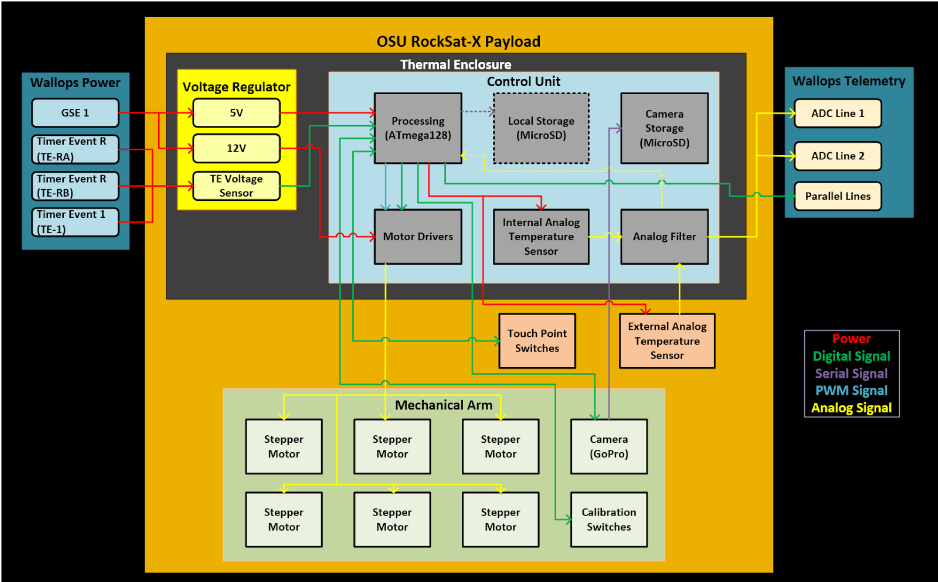
\includegraphics[width=\textwidth]{./images/ProjectDocs/functionalBlockDiagram}

\subsubsection{Flow Diagram}
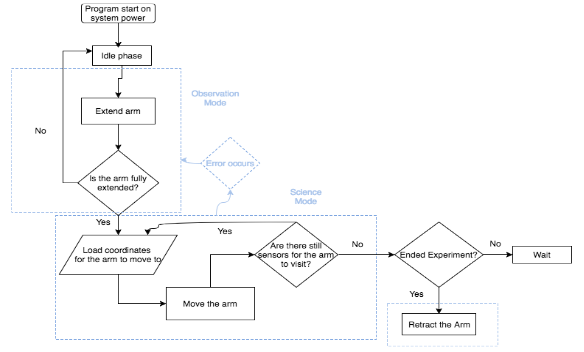
\includegraphics[width=\textwidth]{./images/ProjectDocs/flowDiagram}

\subsubsubsection{Pathing and Automation Subsystem Flow Diagram}
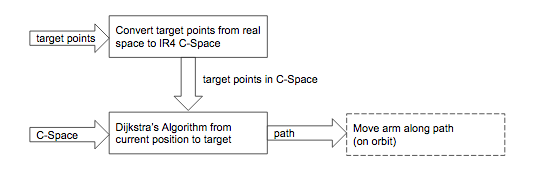
\includegraphics[width=\textwidth]{./images/ProjectDocs/pathingAndAutomationFlow}

\subsection{Hardware Requirements}
Minimum hardware requirements to run the software for the Hephaestus payload include:
\begin{itemize}
	\item{ATmega128 microcontroller}
	\item{USB ASP programmer}
\end{itemize}

\subsection{Installation Instructions}
To install the software on an ATmega128 chip, first ensure it is connected to
the computer with a USB ASP programmer. Then, from the 
\texttt{code/Hephaestus/Hephaestus} directory, run \texttt{make all}
followed by \texttt{make program}.

\subsection{Running Instructions}
The code will immediately begin running once the chip is powered on, and will
continue to run until power is lost.

\subsection{User Guides and Documentation}
\subsubsection{Program Overview}
Hephaestus is a rocketry payload made by Oregon State University for the RockSat-X program. The faculty advisor for this project is Nancy Squires. The involvement of twelve of the project contributors is part of the Senior Design classes. The Senior Design groups include two Mechanical Engineering groups, an Electrical Engineering group, and the Computer Science group. This repository is for project deliverables for the CS Senior Design class as well as any design documents, code, testing, data, and documentation generated by the Computer Science team throughout the 2016/2017 Senior Design year.

Participation and flight in the RockSat-X program is subject to review and approval from the Colorado Space Grant Consortium. Pending this approval, the Hephaestus payload will fly in August of 2017.

\subsubsection{Mission Overview}
The Oregon State University RockSat-X team will demonstrate that an autonomous robotic arm can locate predetermined targets around the payload under microgravity conditions by using precise movements. The technical actions performed by this demonstration will illustrate a proof of concept for creating assemblies, autonomous repairs, and performing experiments in space.

\subsubsection{Repository Contents}
This section will describe the contents and structure of this repository.

\subsubsubsection{Deliverables}
The deliverables directory shall contain all deliverables for the CS Senior Design course. These deliverables are broken up into the term and assignment subdirectories. Assignments will be added through June 2017, at which point the course will conclude.

\subsubsubsection{Design Documents}
The Design Documents directory contains all design documents that we create. These shall be further organized by term and subject, pending need for organization. For the moment this shall be a place for any in progress, partial, or draft items.

\subsubsubsection{Photos}
The Photos directory shall include all photo documentation for the project, including any graphics for promotional use (such as logos or flyers).

\subsubsubsection{Presentations}
The Presentations directory shall include all presentations given by the CS team. This will include all presentations for RockSat-X program design reviews, presentations for promotional purposes, or for fundraising purposes.

\subsubsubsection{Code}
\begin{itemize}
	\item \textbf{CSpace}

	Contains the code for mapping and parsing the configuration space.

	\item \textbf{Drivers}

	Contains the drivers given to us by the Electronics team.

	\item \textbf{Hephaestus}

	Contains all the code written by the Software team to operate the \gls{payload}.

	\item \textbf{SDRead}

	Contains the code to parse telemetry files and display data in a \gls{gui}.
\end{itemize}

\subsubsection{Instructions to build}

\subsubsubsection{Before you build}
Before you can build the code for this project, make sure you have the avr-gcc 
compiler as well as an ATmega128 microchip and programmer. You can obtain a 
copy of the avr-gcc compiler from the 
\href{http://winavr.sourceforge.net/}{WinAVR suite} for Windows, or by 
installing the `avr-libc`, `binutils-avr`, `gcc-avr`, and `avrdude` packages 
from your Linux OS's package repository. In the case of OS X/macOS, ensure that 
you have version 5.11.1 of avrdude installed as the most recent version does 
not work with our implementation. The ATmega128 chip can be purchased from 
\href{https://www.microchip.com/wwwproducts/en/ATMEGA128}{Microchip's website}.
Also, be sure to have a programming board for your ATmega128 chip, which can be 
obtained from the \gls{osu} TekBot store.

\subsubsubsection{Building}
\begin{enumerate}
	\item{Navigate to the \texttt{code/Hephaestus/Hephaestus} directory.}
	\item{Run \texttt{make all} to compile the code.}
	\item{Run \texttt{make program} to program the microcontroller.}
\end{enumerate}
